\chapter{NGS Data \& Quality Assessment}

\section{Initial Goals}

\begin{enumerate}
\item Understand the \textit{Sequencing by Synthesis} Process \& Data Generation \\
\item Understand what errors and artefacts lie within the data \\
\item Learn how to assess the quality of data \& make informed decisions \\
\end{enumerate}

\section{NGS Data Generation}
\begin{steps}
Before we can begin to analyse any data, it is helpful to understand how it was generated.
Whilst there are numerous platforms for generation of NGS data, today we will look at the Illumina \textit{Sequencing by Synthesis} method, which is one of the most common methods in use today.
Many of you will be familiar with the process involved, but it may be worth looking at the following 5-minute video from Illumina: \url{http://youtu.be/womKfikWlxM} 
%As setting up the sound with the VMs can be tricky, it will be easier to view this from your own regular browser.
%Briefly minimise the VM (see Section 1.4), open your regular browser \& please use your headphones if you brought them. \\
\end{steps}

\begin{note}
This video refers to the process \textit{tagmentation}.
This is a relatively recent method for fragmenting \& attaching adaptors to DNA, with an alternative, more traditional method being sonication, poly-adenylation \& attachment of appropriate adaptors in separate steps.
The important concept to note during sample preparation is that the DNA insert has multiple sequences ligated to either end.
These include 1) the \textit{sequencing primers}, 2) index or \textit{barcode} sequences, and 3) the flow-cell binding oligos.
\end{note}

\begin{questions}
Assuming each 'spot' on the flowcell is generated from a unique DNA sequence, there are two important sequencing errors that will occur during this process.
What do you think they might be? \\
\begin{answer}
1) Ligation of the wrong base during sequencing \\
2) Insertions \& deletions \\
It's the same basic errors as normal DNA replication, but without the \textit{in vivo} DNA repair mechanisms.
\end{answer}

Will these errors have a more significant effect if they occur during the sequence detection stage, or during generation of the DNA clones within each cluster? \\
\begin{answer}
The earlier in the process any sequencing errors occur, the higher the degree to which they will be propagated.
If an error occurs during the very first round of amplification, before even bridge amplification, it will be propagated through an entire cluster. \\
\end{answer}

Will all of the individual ssDNA molecules within a spot be amplified perfectly in sync with each other?\\
\begin{answer}
No.  As the reads become longer, the more molecules will get out of sync (i.e. phase) with each other.
As a result the quality scores will drop off towards the end of a read.
\end{answer}
\end{questions}

\section{FASTQ File Format}
\begin{note}
As the sequences are extended during the sequencing reaction, an image is recorded which is effectively a movie or series of frames at which the addition of bases is recorded \& detected.
We mostly don't deal with these image files, but will handle data generated from these in \textit{fastq} format, which can commonly have the file suffix \textit{.fq} or \textit{.fastq}.
As these files are often very large, they will often be zipped using \texttt{gzip} or \texttt{bzip}.
Whilst we would instinctively want to unzip these files using the command \texttt{gunzip}, most NGS tools are able to work with zipped fastq files, and this is usually unnecessary.
This can save considerable hard drive space, which is an important consideration when handling NGS datasets as the quantity of data can easily push your storage capacity to it's limit. \\
\end{note}

\begin{steps}
We should still have a terminal open from the previous section \&, if necessary, use the \texttt{cd} command to make sure you are in the \texttt{\~{}/NGSData/RNASeq/rawData} directory.
The command \texttt{zcat} unzips a file \& prints the output to the terminal, or standard output (\textit{stdout}).
If we did this to these files, we would see a stream of data whizzing past in the terminal, but instead we can just pipe the output of \texttt{zcat} to the command head to view the first 10 lines of a file. \\
\begin{lstlisting}
cd ~/NGSData/RNASeq/rawData
zcat reads1.fq.gz | head -n8
\end{lstlisting}
\end{steps}

\begin{information}
In the above command, we have used a trick commonly used in Linux systems where we have taken the output of one command (\texttt{zcat reads1.fq.gz}) and sent it to another command (\texttt{head}) by using the \textit{pipe symbol} (|).
This is literally like sticking a pipe on the end of a process \& redirecting the output to the input another process.
If you think of things as being like a data factory you can almost visualise it.
There are no limits to the number of commands that you can string together using this trick. 
Additionally, we gave the argument \texttt{-n8} to the command \texttt{head} to ensure that we only printed the first eight lines.\\
\end{information}

\begin{warning}
\large{Don't Panic!!!} \\
\normalsize
If at some stage today you find that the terminal has become unresponsive, or you are seeing an unexpected stream of data fly past, you can abort whichever process is currently running in the terminal by entering \texttt{Ctrl-c}.
This is an instruction to the computer to `kill the current process.' \& you may be surprised at how often this comes in handy.
Even experienced programmers rely on this trick from time to time.
\end{warning}

\begin{note}
In the output from the above terminal command, we have obtained the first 8 lines of the gzipped fastq file.
This gives a clear view of the fastq file format, where each individual read spans four lines.
These lines are:
\begin{enumerate}
\item The read identifier
\item The sequence read
\item An alternate line for the identifier (commonly left blank as just a \texttt{+} symbol acting as a placeholder)
\item The quality scores for each position along the read as a series of ascii text characters.
\end{enumerate}
\end{note}

Let's have a brief look at each of these lines and what they mean.\\

\subsubsection*{The read identifier}
This line begins with an \texttt{@} symbol and although there is some variability, it traditionally has several components.
Today's data have been sourced from an EBI data repository with the identifier \texttt{SRR031714}.
For the first sequence in this file, we have the full identifier \texttt{@SRR031714.1 HWI-EAS299_130MNEAAXX:2:1:785:591/1} which has the following components: \\

\begin{tabular}{|p{5cm} | p{9cm} |}
  \hline
  \texttt{SRR031714.1} & The aforementioned EBI identifier \& the sequence ID within the file. As this is the first read, we have the number 1. NB: This identifier is \textbf{not} present when data is obtained directly from the machine or service provider.\\
  \hline
  \texttt{WHI-EAS299_130MNEAAXX} & The unique machine ID \\
  \hline
  \texttt{2} & The flowcell lane \\
  \hline
  \texttt{1} & The tile within the flowcell lane \\
  \hline
  \texttt{785} & The $x$-coordinate of the cluster within the tile \\
  \hline
  \texttt{591} & The $y$-coordinate of the cluster within the tile \\
  \hline
  \texttt{/1} & Indicates that this is the first read in a set of paired end reads \\
  \hline
\end{tabular}

As seen in the subsequent sections, these pieces of information can be helpful in identifying if any spatial effects have affected the quality of the reads.
By and large you won't need to utilise most of this information, but it can be handy for times of serious data exploration.\\

\begin{steps}
While we are inspecting our data, have a look at the beginning of the second file.
\begin{lstlisting}
zcat reads2.fq.gz | head -n8
\end{lstlisting}
Here you will notice that the information in the identifier is identical to the first file we inspected, with the exception that there is a \texttt{/2} at the end.
This indicates that these reads are the second set in what are known as \textit{paired-end} reads, as were introduced in the above video.
The two files will have this identical structure where the order of the sequences in one is identical to the order of the sequences in the other.
This way when they are read as a pair of files, they can be stepped through read-by-read \& the integrity of the data will be kept intact.
\end{steps}

\subsubsection{The Illumina Chastity Filter}
\begin{information}
It is also worth noting that the reads we've just glanced at come from a version of the Illumina \textit{casava} pipeline which is \textless 1.8, and which is a relatively common format.
The casava version really just describes how old the software on the Illumina machine is \& we don't choose this.
For more recently generated reads where the casava software is \textgreater 1.8 of the casava, there is an additional field in the identifier which indicates whether a read would have \textit{failed} an initial QC check. 
An example of this format would be:
\begin{lstlisting}
@D5B4KKQ1:554:C4YHPACXX:4:1101:1084:2100 1:Y:0:
\end{lstlisting}
Note the ``Y'' in the final fields, which indicates this sequence would have \textbf{failed} QC.
These low-quality reads were automatically removed in earlier versions of the pipeline and were omitted from the fastq file.
However, they are now included with this additional field indicated in the read identifier.
Inspection of this line will enable you to find out which version of the casava pipeline has been used, and whether you need to perform any additional filtering steps to remove low quality reads. 
The tool \texttt{fastq_illumina_filter} is designed to remove these reads for you \& the tool, along with usage instructions can be found at \url{http://cancan.cshl.edu/labmembers/gordon/fastq_illumina_filter/}.\\
\end{information}

\begin{steps}
An alternate set of reads which we'll also explore today is in included in the directory \texttt{\~{}/NGSData/iCLIP/rawData}.
These are immunopreciptated mRNAs and were supplied by some collaborators who'd either forgotten the removal of low-quality reads or had deliberately neglected step to increase read numbers.
Note that these files are not compressed and are essentially plain text files, so we can directly inspect them using the command \texttt{head} instead of decompressing first.\\
\end{steps}

\begin{lstlisting}
cd ~/NGSData/iCLIP/rawData
head -n12 iCLIP_Sample1.fastq
\end{lstlisting}

Note that the header lines follow the format described on the previous page with this additional field at the end of the line.
\begin{questions}
Of the first three reads which have been printed to the terminal above, which one(s) will have failed the chastity filter, and which ones will have passed the filter?\\
\begin{answer}
The first read would have failed (i.e. it is low quality), whilst the other two will have passed.
\end{answer}
\end{questions}

\subsubsection{Quality Scores}
\begin{information}
The only other line in the fastq format that really needs some introduction is the quality score information.
These are presented as single \textit{ascii} text characters for simple visual alignment with the sequence, and each character corresponds to a numeric value, which is the quality score.
In the ascii text system, each character has a numeric value which we can interpret as an integer.
Head to the website with a description of these at \url{http://en.wikipedia.org/wiki/ASCII#ASCII_printable_code_chart}.\\

The first 31 characters are non-printable \& contain things like end-of-line marks and tab spacings, and note that the first printable character after the space is `!' which corresponds to the value 33.
In short, the values 33-47 are symbols like !, \", \#, \$ etc, whereas the values 48-57 are the characters 0-9.
Next are some more symbols (including @ for the value 64), with the upper case characters representing the values 65-90 \& the lower case letters representing the values 97-122.\\

In the line of quality scores for the first read in the iCLIP sample above, the first character is ``=", so this base has a quality score of 61.
The second symbol in this line is``D", so the second base has a quality score of 68.
\end{information}

\subsubsection{The PHRED +33/64 Scoring System}
\begin{information}
Now that we understand how to turn the quality scores from an ascii character into a numeric value, we need to know what these numbers represent.
The two main systems in common usage are PHRED +33 and PHRED +64 and for each of these coding systems we either subtract 33 or 64 from the numeric value associated with each ascii character to give us a PHRED score.
As will be discussed later, this score ranges between 0 and about 41.\\

The PHRED system used is determined by the software installed on the sequencing machine, with early machines using PHRED + 64 (casava \textless 1.5), and more recent machines tending to use PHRED + 33.
For example, in PHRED +33, the @ symbol corresponds to Q = 64 - 33 = 31, whereas in PHRED +64 it corresponds to Q = 64 - 64 = 0. \\
\end{information}

\begin{minipage}{\textwidth}

The following table demonstrates the comparative coding scale for the different formats: \\

\scriptsize
\texttt{...............................IIIIIIIIIIIIIIIIIIIIIIIIIIIIIIIIIIIIIIIII...................... \\
.................................\textbf{J}JJJJJJJJJJJJJJJJJJJJJJJJJJJJJJJJJJJJJJ...................... \\
LLLLLLLLLLLLLLLLLLLLLLLLLLLLLLLLLLLLLLLLLL.................................................... \\
!"\#\$\%\&'()*+,-./0123456789:;\textless =\textgreater?@ABCDEFGHIJKLMNOPQRSTUVWXYZ[\textbackslash]\^{}_`abcdefghijklmnopqrstuvwxyz\{|\}\~{}} \\
\texttt{
~~|~~~~~~~~~~~~~~~~~~~~~~~~~|~~~~|~~~~~~~~|~~~~~~~~~~~~~~~~~~~~~~~~~~~~~~|~~~~~~~~~~~~~~~~~~~~~|~\\
~33~~~~~~~~~~~~~~~~~~~~~~~~59~~~64~~~~~~~73~~~~~~~~~~~~~~~~~~~~~~~~~~~~104~~~~~~~~~~~~~~~~~~~126~\\
~ \\
I - Illumina 1.3+ Phred+64,  raw reads typically (0, 40) \\ 
J - Illumina 1.5+ Phred+64,  raw reads typically (3, 40) \\
L - Illumina 1.8+ Phred+33,  raw reads typically (0, 41) \\
}
%\normalsize
\end{minipage}

\begin{questions}
Have a look at the quality scores in the RNA-Seq data. 
Which coding system do you think has been used for the RNA-Seq reads that we have? \\
\begin{answer}
PHRED+33. 
The presence of values between `!' \& `?' gives this away.\\
\end{answer}
In the PHRED +33 coding system, the character `@' is used.
Can you think of any potential issues this would cause when searching within a fastq file? 
(Hint: Consider the sequence identifier rows)\\
\begin{answer}
It is also included as the beginning of each sequence identifier.
If located at the beginning of a string of quality scores, this may be misunderstood as a sequence identifier.
This is good to keep in mind when writing custom code for searching fastq files.
\end{answer}
\end{questions}

\subsubsection{Interpretation of PHRED Scores}

\begin{information}
All NGS platforms have non-zero error rates during the sequencing process (\url{http://www.molecularecologist.com/next-gen-table-3c-2014/}), and the quality scores are related to the probability of calling an incorrect base.
The PHRED scoring system predates NGS technologies \& is based on whether the wavelength from one specific base is clearly dominant through the formula
\begin{equation}
  \label{eq:PHRED}
  Q = -10 log_{10} P
\end{equation}
where $P$ is the probability of calling the incorrect base. \\
\end{information}

This is more easily seen in the following table: \\
\begin{center}
\begin{tabular}[h]{|p{3cm} p{5cm} p{3cm}|}
\hline
\textbf{PHRED Score} & \textbf{Probability of Incorrect Base Call} &
\textbf{Accuracy of Base Call} \\
\hline
0 & 1 in 1 & 0\% \\
10 & 1 in 10 & 90\% \\
20 & 1 in 100 & 99\% \\
30 & 1 in 1000 & 99.9\% \\
40 & 1 in 10000 & 99.99\% \\
\hline
\end{tabular}
\end{center}

\begin{note}
As each base is added, the light wavelength associated with each base (i.e. the colour) is detected.
In theory, there should only be one colour observed, but in reality there will always be a residual signal from the other bases.
The following chromatogram based on the traditional Sanger sequencing methods demonstrates this well (Source: \url{http://seqcore.brcf.med.umich.edu}.\\
\end{note}

\begin{figure}[h!]
  \centering
    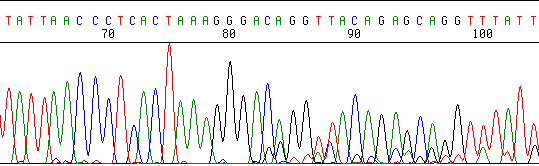
\includegraphics[width=0.8\textwidth]{clonesite}
\end{figure}

Note that early in this sequence, the colour peaks are clear but with small residual peaks of background signal.
These peaks would receive high PHRED scores.
Around position 83 however, the peaks become less obvious and any corresponding PHRED score would be lower.
This basic principle is applied on a massively parallel scale during the generation of NGS data.\\

\begin{questions}
A common threshold for inclusion of a sequence is that all bases must have a Q score >20.
Considering the millions of sequences obtained from a flowcell, do you think that NGS data is likely to be highly accurate?\\
\begin{answer}
This is really just a point for everyone to ponder.
People should be encouraged to realise that NGS data will have a lot of errors...
\end{answer}
\end{questions}

\clearpage
\section{Using fastqc}
\begin{steps}
Removal of low-confidence base calls is an important part of any NGS analysis, and we can begin this process by checking the quality of libraries using the tool \texttt{fastqc}.
As with all programs on the command line, we need to see how it works before we use it.
The following command will open the help file in the \texttt{less} pager which we used earlier.
To navigate through the file, use the \textless spacebar\textgreater ~to move forward a page, \textless \texttt{b}\textgreater ~to move back a page \& \textless \texttt{q}\textgreater ~to exit the manual. \\
\begin{lstlisting}
fastqc -h | less
\end{lstlisting}
\end{steps}

\begin{note}
Fastqc will create an html report on each file you submit, which can be opened from any web browser, such as \texttt{firefox}
As seen in the help page, \texttt{fastqc} can be run from the command line or from a graphic user interface (GUI).
Using a GUI is generally intuitive, so today we will look at the command line usage, as that will give you more flexibility \& options going forward.
Some important options for the command can be seen in the manual.\\
\end{note}
\begin{steps}
As you will see in the manual, setting the \texttt{-h} option as above will call the help page.
Look up the following options to find what they mean. \\
\begin{center}
\begin{tabular}[h]{|p{4cm}|p{8cm}|}
  \hline
  \textbf{Option} & \textbf{Usage} \\
  \hline
  -o & \\
   & \\
   \hline
  -t & \\
   & \\
   \hline
   -{}-casava & \\
   & \\
   \hline
\end{tabular}
\end{center}
\end{steps}

\begin{steps}
As we have two RNA-Seq files, we will first need to create the output directory, then we can run \texttt{fastqc} using 2 threads which will ensure the files are processed in parallel.
This can be much quicker when dealing with large experiments.
\begin{lstlisting}
cd ~/NGSData/RNASeq/rawData
mkdir -p ~/QC/RNASeq/rawData
fastqc -o ~/QC/RNASeq/rawData -t 2 reads1.fq.gz reads2.fq.gz
\end{lstlisting}
It's probably a good idea to scribble a note next to each line if you didn't understand what you did.
If you haven't seen the command \texttt{mkdir} before, check the help page 
\begin{lstlisting}
man mkdir
\end{lstlisting}
\end{steps}

\begin{steps}
The above command gave both files to fastqc, told it where to write the output (\texttt{-o \~{}/QC}) \& requested two threads (\texttt{-t 2}). 
The reports are in the html files, with all of the plots stored in the zip files. 
To look at the QC report for each file, we can use \texttt{firefox}.
\begin{lstlisting}
cd ~/QC/RNASeq/rawData
ls -lh
firefox reads1.fq_fastqc.html reads2.fq_fastqc.html &
\end{lstlisting}
The left hand menu contains a series of click-able links to navigate through the report, with a quick guideline about each section given as a tick, cross of exclamation mark.
\end{steps}

\begin{note}
Two hints which may make your inspection of these files easier are:
\begin{enumerate}
	\item To zoom out in \texttt{firefox} use the shortcut Ctrl-. Reset using Ctrl0 and zoom in using Ctrl+
	\item You can open these directly from a traditional directory view by double clicking on the .html file.
\end{enumerate}
If your terminal seems busy after you close \texttt{firefox}, use the 'Ctrl C' shortcut to stop whatever is keeping it busy
\end{note}

\begin{questions}
How many reads are there in both files?\\
\begin{answer}
  2500000 \\
\end{answer}
How long are the reads in these files?\\
\begin{answer}
  37bp \\
\end{answer}
\end{questions}

\section{Interpreting the FASTQC Report}
\begin{note}
As we work through the QC reports we will develop a series of criteria for filtering and cleaning up our files.
There is usually no perfect solution, we just have to make the best decisions we can based on the information we have.
Some sections will prove more informative than others, and some will only be helpful if we are drilling deeply into our data.
Firstly we'll just look at a selection of the plots.
We'll investigate some of the others with some `bad' data later.
\end{note}

\subsubsection*{Per Base Sequence Quality}
\begin{steps}
Both of the files should be open in \texttt{firefox} in separate tabs.
Perform the following steps on both files.
Click on the \texttt{Per base sequence quality} hyperlink on the left of the page \& you will see a boxplot of the QC score distributions for every position in the read.
This is the main plot that researchers will look at for making informed decisions about later stages of the analysis.
\end{steps}

\begin{questions}
What do you notice about the QC scores as you progress through the read? \\
\begin{answer}
They clearly drop off as the read extends.\\
\end{answer} 
\end{questions}

We will deal with trimming the reads in a later section, but start to think about what you should do to these reads to ensure the highest quality in your final alignment \& analysis.

\paragraph{Per Tile Sequence Quality}
This section just gives a quick visualisation about any physical effects on sequence quality due to the tile within the each flowcell.
For the first file, you will notice an even breakdown in the quality of sequences near the end of the reads across all tiles.
In our second QC report, you will notice a poor quality around the 25th base in the 2nd (or 3rd) tile.
Generally, this would only be of note if drilling deeply to remove data from tiles with notable problems.
Most of the time we don't factor in spatial effects, unless alternative approaches fail to address the issues we are dealing with.

\paragraph*{Per Sequence Quality Scores}
This is just the distribution of average quality scores for each sequence.
There's not much of note for us to see here.

\paragraph{Per Base Sequence Content}
This will often show artefacts from barcode sequences or adapters early in the reads, before stabilising to show a relatively even distribution of the bases.

\paragraph{Sequence Duplication Levels}
This plot shows about what you'd expect from an RNA-Seq experiment.
There are a few duplicated sequences (rRNA?, highly expressed genes? etc.) and lots of unique sequences represented the diverse transcriptome.
This is only calculated on a small sample of the library for computational efficiency and is just to give a rough guide if anything unusual stands out

\paragraph{Kmer Content}
Statistically over-represented sequences can be seen here \& often they will overlap. 
In our first plot, the some sequences derive from the same motif, and are the extracts of the same longer sequence, just shifted along one base.
No information is given as the source of these sequences, and you would expect to see barcode sequences or motifs that correspond to any digestion protocols here.
This is a plot that can cause significant confusion, but can alert you to any unexpected sequence-based problems in your data.

\subsection{Some Flawed Data}
Let's run \texttt{fastqc} \& inspect the iCLIP dataset, which is a version of RNA-Seq data where the RNA has been pulled down via IP after cross-linking to an RNA-associated protein.

\begin{lstlisting}
mkdir -p ~/QC/iCLIP/rawData
cd ~/NGSData/iCLIP/rawData
fastqc -o ~/QC/iCLIP/rawData -t 2 iCLIP_Sample1.fastq iCLIP_Sample2.fastq
cd ~/QC/iCLIP/rawData
firefox iCLIP_Sample1_fastqc.html iCLIP_Sample2_fastqc.html &
\end{lstlisting}

There are several things to note about these reports.
Firstly, we know from inspection that these fastq libraries contain reads which have failed the Illumina Chastity filter.
We would expect these to show up in the \textit{Basic Statistics} table, but they don't by default.

\begin{questions}
How would we know that there are low quality reads here if the Illumina flag is ignored?\\
\begin{answer}
The overall lower distribution of the quality scores should raise a red flag to us. \\
\end{answer}
\end{questions}

To see how these reads look without the flagged reads, we can turn on the \texttt{-{}-casava} option when running \texttt{fastqc}.
You can ignore any warning messages you receive about not looking like part of a CASAVA group.

\begin{lstlisting}
cd ~/NGSData/iCLIP/rawData
fastqc --casava -o ~/QC/iCLIP/rawData -t 2 iCLIP_Sample1.fastq iCLIP_Sample2.fastq
cd ~/QC/iCLIP/rawData
firefox iCLIP_Sample1_fastqc.html iCLIP_Sample2_fastqc.html &
\end{lstlisting}

\begin{information}
Note that the above code will have over-written the original QC reports.
As this second analysis is the best approach, this is actually OK at this point.
However. this can be a common pitfall when running an analysis, which is why we will often record our analysis as a script.
That way we have a record of what we have done and know exactly what options we have set for a process.
\end{information}


\paragraph{Adapter Contamination}
Go to the over-represented sequences section for Sample1.
There seem to be a large number of over-represented sequences here which are not listed as matching any known sequences.
Scanning through these manually is near impossible and solving this may take some leg work.
Shift over to the same section in Sample2 and you will notice about 23\% of sequences seem to contain an Illumina Paired End PCR Primer.
The next line also contains matches to this but with some indels. \\

Now head to the \textit{Adapter Content} section of each report \& consider what we are seeing here.
By the time you reach the 60th nucleotide in the reads from Sample1, this plot tells you that $>50$\% of reads contain matches to the Illumina Universal Adapter.


\subsection{Some More Example Reports}
We'll actually try to clean the iCLIP dataset up in the next chapter, but for now let's just head to another sample plot at \url{http://www.bioinformatics.babraham.ac.uk/projects/fastqc/bad_sequence_fastqc.html}


\paragraph{Per Base Sequence Quality}
Looking at the first plot, we can clearly see this data is not as high quality as the one we have been exploring ourselves.

\begin{questions}
Consider that the minimum sequence length required for confidently obtaining unique alignments is >20bp.
Two approaches to this data might be to only include high quality sequences, or to trim the low quality bases from the ends and use shorter reads for downstream analysis.
What would be the consequences of either approach? \\
\begin{answer}
If we excluded low quality sequences, we would throw away a large amount of data.
Depending on the question we are asking of the data, this may render our experiment meaningless or may help us find more accurate results.
Context is everything. \\
If we trimmed the reads, we may retain a larger number of them, but more may map to non-unique locations in the reference.
Once again, context is everything.\\
\end{answer}
\end{questions}

\paragraph{Per Tile Sequence Quality}
Some physical artefacts are visible \& some tiles seem to be consistently lower quality.
Whichever approach we take to cleaning the data will more than likely account for any of these artefacts.
Sometimes it's just helpful to know where a problem has arisen.

\paragraph{Overrepresented Sequences}
Head to this section of the report \& scan down the list.
Unlike our sample data, there seem to be a lot of enriched sequences of unknown origin.
There is one hit to an Illumina adaptor sequence, so we know at least one of the contaminants in the data.
Note that some of these sequences are the same as others on the list, just shifted one or two base pairs.
A possible source of this may have been non random fragmentation.

\paragraph{Kmer Content}
\begin{questions}
Do you notice anything unusual about this plot?\\
\begin{answer}
The K-mers are present at the end of the reads.
Was this a problem with sample preparation? 
Do these map to barcodes, adaptors or primers at the other end of the reads? \\
\end{answer}
\end{questions}

\begin{information}
Interpreting the various sections of the report can take time \& experience.
A description of each of the sections is available from the \texttt{fastqc} authors at \url{http://www.bioinformatics.babraham.ac.uk/projects/fastqc/Help/}
\end{information}

\begin{bonus}
Another interesting report is available at \url{http://www.bioinformatics.babraham.ac.uk/projects/fastqc/RNA-Seq_fastqc.html}
Whilst the quality scores generally look pretty good for this one, see if you can find a point of interest in this data.
This is a good example, of why just skimming the first plot may not be such a good idea.
\end{bonus}

\begin{advanced}
In our dataset of two samples it is quite easy to think about the whole experiment \& assess the overall quality.
What about if we had 100 samples? 
Each .zip archive contains text files with the information which can easily be parsed into an overall summary. \\

Whilst this will require low-level scripting skills to perform on an experiment, we can quickly look at two of the important files today.
The overall summary in terms of PASS/FAIL is contained in the `summary.txt' file within the archive.
Open this file in the \texttt{less} pager, and once you've had a look type \texttt{q} to quit, as we have become familiar with.
First make sure you are in the correct directory, then inspect these files using \texttt{less}.
\begin{lstlisting}
cd ~/QC/RNASeq/rawData
unzip -oc reads1.fq_fastqc.zip '*summary.txt' | less
\end{lstlisting}

The raw numbers for each of the sections are in the file fastqc_data.txt.
Page through the file, until you lose interest then quit the pager.
\begin{lstlisting}
unzip -oc reads1.fq_fastqc.zip '*fastqc_data.txt' | less
\end{lstlisting}

We can also extract any specific image file for compiling into a pdf, or find whatever we need by using these ideas.
This makes handling the data for a large experiment much simpler.
There are plenty of hints online for how to write a \textit{shell script}, or alternatively, attend one of our scripting workshops.
\end{advanced}

\section{Further Reading}
An excellent article which deals with some of the issues around data quality is:

Zhou, X and Rokas, A. (2014). \textit{Prevention, diagnosis and treatment of high-throughput sequencing data pathologies.} Molecular Ecology 23, 1679-1700.

This has been included on your VM as the file QC.pdf \& contains many examples of good data and low quality data, as well as a detailed discussion.
If you feel like you are running ahead of schedule, or if you finish early it may be a good opportunity to download \& read through the article.
The workflow given at the end may also be particularly useful.